\documentclass[14pt]{extreport}
\usepackage{gost}
\usepackage{minted}

\addto\captionsrussian{\def\refname{Список используемой литературы}}

\begin{document}
\includepdf[pages={1}]{titulnyy_list_oznakomitelnaya_praktika.pdf}


\tableofcontents

\intro

Для современного математика и исследователя важны не только навыки решения задач аналитически и численно на бумаге или доске, но также и умение пользоваться современными пакетами компьютерной алгебры, такими как Euler Math Toolbox или Mathcad, а также умение представить полученные результаты  в определенном стиле и формате. Определенным стандартом оформления работы математика де-факто является издательская система LaTeX.     

В данной работе я получаю практические навыки по двум направлениям, востребованным в современных условиях: использование пакета компьютерной алгебры на примере Euler Math Toolbox, а также верстка математического текста, используя издательскую систему LaTeX. В качестве источника задач мною выбрано издание <<Конспект лекций по высшей математике: полный курс>>  Д. Т. Письменный. - 4-е изд. - М.: Айрис-пресс, 2006. - 608 с.: ил. - (Высшее образование).





\chapter{HTML: База}

\section{HTML}

HyperText Markup Language (гипертекст маркап лэнгуидж) - язык разметки гипертекста. В этой аббревиатуре нам интересно слово "разметка".

Разметка - что это вообще такое? Представь, что ты передаёшь текст по сети. Как сделать в тексте заголовок? Выделить абзац? Подчеркнуть слово? Самый простой вариант - пометить начало и конец выделяемого фрагмента условными метками. Например:
\begin{minted}{HTML}
<заголовок>HTML</заголовок>
<полужирный>HyperText Markup Language</полужирный> <курсив>(гипертекст маркап лэнгуидж)</курсив> - язык разметки гипертекста.
\end{minted}
Это разметка.




\section{Теги}
Тег — это синтаксическая единица языка HTML, которая выделяет или создаёт элемент. Это набор символов, с помощью которого браузер понимает, где элемент создается, начинается и заканчивается. Есть 2 вида тегов: двойные и одинарные.

Двойные теги
Двойные теги показывает начало и конец элемента. Начало элемента обозначается открывающим тегом \mintinline{latex}{<…>}, а конец - закрывающим \mintinline{latex}{</…>}.

Двойной тег обязательно должен быть закрыт. Даже несмотря на то, что современные браузеры умеют в некоторых случаях понимать разметку без закрытых тегов, лучше всегда закрывать их.

Одинарные теги
Одинарные теги просто не имеют пары. Примеры: тег переноса строки \mintinline{latex}{<br>} или горизонтальной линии  \mintinline{latex}{<hr>}.

Старые браузеры требовали закрывать одинарные теги: \mintinline{latex}{<br />}, сейчас таких браузеров практически не осталось и допустимо использовать оба варианта синтаксиса.



\section{Атрибуты}
Атрибуты — это свойства тега. С помощью них мы задаём параметры тега.

Сразу возьмём пример: тег \mintinline{latex}{<a>} — ссылка. Для задания адреса, куда будет вести эта ссылка, нам понадобится атрибут \mintinline{latex}{href}. Вот так будет выглядеть ссылка на страницу ITC Вконтакте:
\begin{minted}{html}
<a href="https://vk.com/itc.digital">ITC Вконтакте</a>
\end{minted}
Атрибут указывается внутри тега, значение атрибута указывается внутри кавычек. Атрибуты отделяются друг от друга пробелами. Пример ссылки на страницу ITC, которая откроется в новой вкладке:

\begin{minted}{html}
<a href="https://vk.com/itc.digital" target="_blank">ITC Вконтакте</a>
\end{minted}

У атрибута может не быть значения, тогда наличие атрибута включает какой-то параметр, а отсутствие - отключает. Например, атрибут \verb disabled. Если кнопке \mintinline{latex}{<button>} задать атрибут \mintinline{latex}{disabled}, она станет серой и на неё невозможно будет нажать.

\begin{minted}{html}
<button disabled>Нельзя нажимать</button>
\end{minted}

\begin{figure}[H]
\centerline{
\includegraphics[width=1.0\linewidth]{pics_practice/disabled_button.png}}
\caption{}
\label{}
\end{figure}




\section{Особенности интерпретации HTML}
При преобразовании HTML-кода в веб-страничку есть некоторые особенности, в которых мы сейчас разберёмся.

\emph{Перенос строки только через тег.}

Возможно, у тебя возник вопрос, зачем нужен тег переноса строки, если можно просто нажать энтер. Дело в том, что HTML воспринимает перенос строки как пробел. Это нужно потому, что редакторы кода не переносят строки, которые не помещаются в экран - так удобнее писать код. Поэтому чтобы длинный текст влезал в экран, в коде ставятся переносы строки, которые не нужны, когда страница показывается в браузере.

\emph{Несколько пробелов, идущих подряд, считаются за один.}

Это происходит по той же причине, что и с переносом строки. Так просто удобнее форматировать код в редакторе. Из-за того, что теги вкладываются друг в друга, для удобного восприятия кода вложенность показывают отступами - пробелами. Пример:

\begin{figure}[H]
\centerline{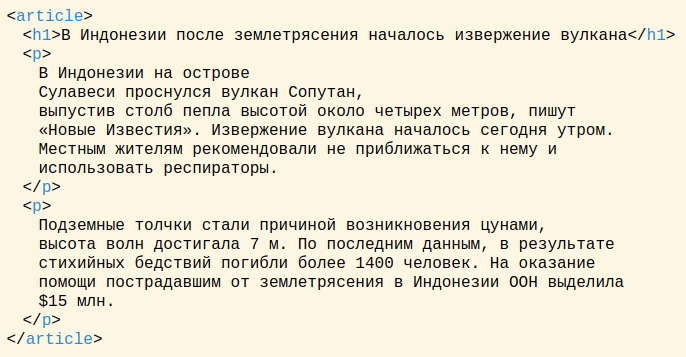
\includegraphics[width=1.0\linewidth]{pics_practice/interpretation_HTML.png}}
\caption{}
\label{}
\end{figure}

\emph{Произвольный регистр.}

\mintinline{latex}{<br>} даст такой же результат, что и \mintinline{latex}{<BR>}, и \mintinline{latex}{<Br>}, и \mintinline{latex}{<bR>}. Несмотря на это, писать разметку лучше в нижнем регистре - это негласное правило.

\emph{Перенос строки в теге.}

При определении тега и его атрибутов можно переносить строку. Это полезно для длинных определений.
Например, для этого изображения:
\begin{minted}{html}
<img
  src="http://example.com/cat.jpg"
  title="Мурка"
  alt="Рыжая кошка валяется в снегу"
  width="640"
  height="480"
>
\end{minted}





\chapter{HTML: Основные элементы}

\section{Структура HTML-документа}

Структура HTML документа - скелет, на основе которого строится вся страница:
\begin{minted}{html}
<!DOCTYPE html>
<html>
  <head>
    <meta charset="utf-8">
    <title>Страница</title>
  </head>
  <body>
    <h1>...</h1>
    <p>...</p>
  </body>
</html>
\end{minted}

\textbf{<!DOCTYPE>}

Первым тегом в любом HTML документе должен идти тег <!DOCTYPE>. Он говорит браузеру, по какому стандарту написана страница. На рассвете веба HTML существовал в разных несовместимых версиях, поэтому для их одновременной поддержки нужно было указывать версию явно. Сейчас все пришли к одному стандарту - HTML5. Поэтому для всех сайтов, которые создаются сегодня, нужно указывать <!DOCTYPE html> - так обозначается HTML5.

\textbf{<html>}

Вторым тегом идет <html> - контейнер, который содержит два тега - \mintinline{latex}{<head>} и \mintinline{latex}{<body>}. HTML-страница должна заканчиваться закрытым тегом \mintinline{latex}{</html>}.

\textbf{<head>}

В теге <head> хранится информация о странице. Здесь указывают кодировку \mintinline{latex}{<meta charset="...">}, имя страницы \mintinline{latex}{<title>...</title>}, специальную информацию для поисковиков, а ещё тут подключаются стилевые файлы и скрипты.

Тег \mintinline{latex}{<head>} не отображается. Его цель — сказать браузеру информацию о странице.

\textbf{<body>}

В теге \mintinline{latex}{<body>} размещается весь контент страницы, который пользователь увидит в браузере.





\section{Практика: создание веб-страницы}
Создаем файл и называем его \textbf{index.html}. Вставляем туда структуру HTML-страницы из предыдущего урока:
\begin{figure}[H]
\centerline{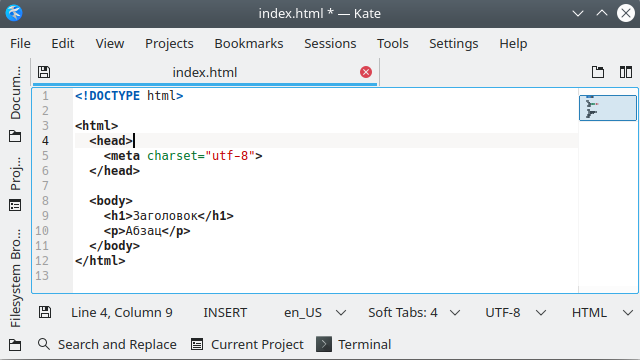
\includegraphics[width=1.0\linewidth]{pics_practice/index_html.png}}
\caption{}
\label{}
\end{figure}
Сохраняем файл и открываем в браузере. Видим:
\begin{figure}[H]
\centerline{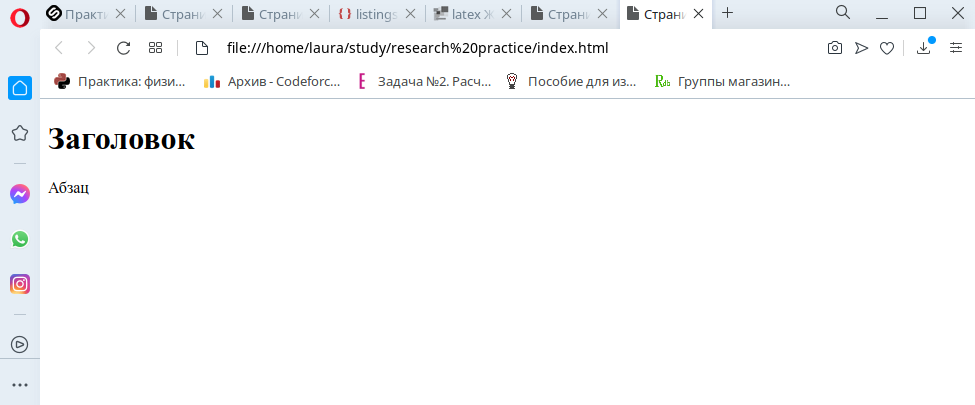
\includegraphics[width=1.0\linewidth]{pics_practice/header.png}}
\caption{}
\label{}
\end{figure}




\section{Редакторы кода}

Разработчики пишут код в специальных редакторах. Они отличаются назначением. Остальные отличия почти всегда вытекают из него. Существует несколько редакторов кода, которые подходят для веб-разработки. Мы рассмотрим несколько из них и порекомендуем два (один из них только для слабых компьютеров). 
Notepad++ - для ветеранов.
Боевая классика. Ветеран среди редакторов кода, в бородатые года считался самым популярным у веб-разработчиков. Сегодня его в основном используют ностальгирующие консерваторы.

Sublime Text -  для слабых компьютеров.
Самый популярный редактор кода у разработчиков на Python. Для веб-разработки тоже подходит. Довольно быстро работает, неплохо выглядит и кастомизируется, имеет несколько полезных плагинов. В целом неплох, но для веб-разработчика есть более подходящий софт. Рекомендуем использовать его только если у тебя слабый компьютер.

Atom - для хипстеров.
Хороший редактор кода, заточенный под веб-разработку. Много тем оформления, плагинов. Работает на веб-технологиях, поэтому если ты планируешь развиваться дальше и изучать JavaScript, то в дальнейшем сможешь писать свои расширения. Его минус - скорость работы. Поэтому его использовать не рекомендуем.

Visual Studio Code - рекомендация.
Не путай с Visual Studio. Редактор кода для веба от Microsoft. По сути, это более быстрый аналог Atom. Он имеет все те же самые плюсы, что и Atom, но работает ощутимо быстрее. Из минусов только майкрософтовый тоталитарный внешний вид, который легко изменить, установив другую тему оформления.



\section{Элементы и их виды}

Элементы - то, что создаётся тегами. Можно сказать, что теги это текстовое представление элементов. Элементы бывают двух видов:

\emph{Блочные элементы}

Составляют структуру страницы.

Особенности:
\begin{itemize}
\itemблоки располагаются друг под другом по вертикали
\itemзапрещено вставлять блочный элемент внутрь строчного
\itemзанимают всё допустимое пространство по ширине
\itemвысота вычисляется автоматически, исходя из содержимого
\end{itemize}

Примеры:
\begin{itemize}
\itemабзацы \mintinline{latex}{<р>}
\itemсписки: маркированные (с маркером) \verb <ul> и нумерованные (с числами) \mintinline{latex}{<ol>}
\itemзаголовки: от первого уровня \verb <h1> до шестого уровня \mintinline{latex}{<h6>}
\itemстатьи \mintinline{latex}{<article>}
\itemразделы \mintinline{latex}{<section>}
\itemдлинные цитаты \mintinline{latex}{<blockquote>}
\itemблоки общего назначения  \mintinline{latex}{<div>}
 \end{itemize}

\emph{Строчные элементы}

Используются для форматирования текстовых фрагментов. Обычно содержат одно или несколько слов.

Особенности:
\begin{itemize}
\itemэлементы, идущие подряд, располагаются на одной строке и переносятся на другую при необходимости
\itemвнутрь допустимо вставлять текст или другие строчные элементы, помещать блочные элементы - запрещено
\end{itemize}

Примеры:
\begin{itemize}
\itemссылки \mintinline{latex}{<a>}
\itemвыделенные слова \mintinline{latex}{<em>}
\itemважные слова \mintinline{latex}{<strong>}
\itemкороткие цитаты \mintinline{latex}{<q>}
\itemаббревиатуры \mintinline{latex}{<abbr>}
\end{itemize}




\section{Списки}

В HTML существует три вида списков:

\emph{Маркированный}

Список из неупорядоченных элементов.

Состоит из двух тегов:
\begin{itemize}
\item \verb <ul> (unordered list) - тег начала и конца списка
\item \verb <li> (list item) - пункт списка
\end{itemize}






\conclusions

Я достигла целей, которые были поставлены передо мной в данной ознакомительной практике, а именно познакомилась со способами нахождения пределов, производных, а также решением сопутствующих задач в пакете компьютерной алгебры Euler Math Toolbox. Также я овладела принципами верстки в издательской системе LaTeX.  В процессе работы над данным документом я пользовалась официальной документацией, а также навыками решения модельных задач, полученными ранее в курсе математического  анализа. Сложнее всего для меня было освоить синтаксис элементов оформления математического текста в системе LaTeX. Частично мне помог в решении этой проблемы пакет TeXworks с подсветкой синтаксиса.  

Отдельную задачу представляла установка необходимого программного обеспечения в дистрибутиве Linux - Ubuntu 18.04. Файлы с исходным кодом LaTeX я версионировала, используя систему контроля версий git, разместив репозиторий на ресурсе github по адресу https://www.github.com/laurardaz/practice. С помощью этого удалось фиксировать промежуточные версии работы, что сделало нахождение ошибок при верстке легким и быстрым. 

Полученные мной навыки я считаю полезными и перспективными для моего последующего обучения, прохождения практики, а также трудоустройства.  

\newpage
 

 
%далее сам список используевой литературы
\begin{thebibliography}{}
    \bibitem{litlink1}  Письменный Д. Т.  -  "Конспект лекций по высшей метематике: полный курс" - 4-е изд. - М.: Айрис-пресс, 2006.- 608 с.: ил. - (Высшее образование).
    \bibitem{overleaf.com}  LaTeX Basics [Электронный ресурс]. - https://www.overleaf.com/learn
    \bibitem{other-link-name} Euler Math Toolbox Tutorials [Электронный ресурс]. -  http://www.euler-math-toolbox.de/tutorials.html
    \bibitem{overleaf.com}Online LaTeX Editor [Электронный ресурс]. - https://www.overleaf.com/
    \bibitem{overleaf.com}LaTeX:Symbols [Электронный ресурс]. - https://artofproblemsolving.com/wiki/

index.php/LaTeX:Symbols

\end{thebibliography}

\end{document} 
